\documentclass[a4paper,11pt]{article}
\usepackage[left=1.5cm, right=1.5cm, top=2cm, bottom=1.5cm]{geometry}
\usepackage{graphicx}
\usepackage{amssymb}
\usepackage{amsmath}
\usepackage{wrapfig}

\begin{document}
\title{\LARGE{\textbf{ECEN 204 Lab 4}\\Bipolar Junction Transistors}}
\author{Niels Clayton : 300437590\\ \textbf{Lab Partner: }Nickolai Wolfe}
\date{September 16, 2019}
\maketitle
\hrule

\section{Bipolar Junction Transistor (BJT) Measurements}

\begin{center}
\begin{tabular}{|c|c|c|}  
\hline
 Path Tested & Resistance  & Diode Voltage\\
\hline
Base \(\displaystyle \rightarrow \) Collector & 481k\(\displaystyle \Omega \) & 0.703V\\
Collector \(\displaystyle \rightarrow \) Base & \(\displaystyle \infty  \) & Na\\
\hline
Base \(\displaystyle \rightarrow \) Emitter & 488k\(\displaystyle \Omega \) & 0.698V\\
Emitter \(\displaystyle \rightarrow \) Base & \(\displaystyle \infty  \) & Na\\

\hline
\end{tabular}
\end{center}

\begin{wrapfigure}{r}{0.3\textwidth}
\vspace{-40pt}
\begin{center}
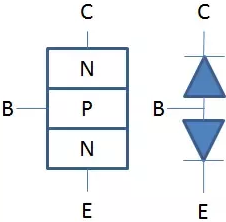
\includegraphics[width=0.2\textwidth]{BJT-diode.png}
\end{center}
\vspace{-18pt}
\caption{BJT Diode Model}
\end{wrapfigure}

From these measurements, it can be deduced that a BJT has a similar internal construction to 2 diodes placed in opposite directions as shown in figure 1. Using this model, it would be expected to measure voltage drops of around 0.7V in the forward bias direction's of both diodes (Base $\rightarrow$ Collector \& Base $\rightarrow$ Emitter), and for there to be a measurable resistance across the diode. However when placing the diodes in reverse bias (Collector $\rightarrow$ Base \& Emitter $\rightarrow$ Base), the resistance should be near infinite. Both of these expected trends can be observed in the above table of measurements:

\section{Current Limiting Resistors}

In our constructed circuit, there were 2 current limiting resistors, one placed between $V_{BB}$ and the base, and the other between $V_{CC}$ and the collector. The purpose of these resistors are to limit the maximum current than can flow from both the base to the emitter, and the collector to the emitter. This is done in order to stop the BJT from exceeding its maximum ratings. 

Using $4.7k\Omega$ resistor attached to the base, and a $1k\Omega$ resistor attached to the collector, and assuming an ideal transistor, we can calculate the maximum $I_{B}$ and $I_{C}$.

$$I_B =  \frac{V_{BB}}{R} = \frac{5}{4.7k} = 1.06mA$$
$$I_C =  \frac{V_{cc}}{R} = \frac{10}{1k} = 10mA$$

\pagebreak
\section{Current Gain}

The current gain of the BJT is defined by the input collector current $I_C$ vs the input base current $I_B$. This was measured both using a transistor tester, and by measuring the $I_C$ and $I_B$ with different current limiting resistors. \\

The outputs are as follows:\\\\
Using transistor tester: $\beta = 440$\\
Using lab measurements: $\beta = 391$\\
\begin{wrapfigure}{r}{0.6\textwidth}
\vspace{-110pt}
\begin{center}
\fbox{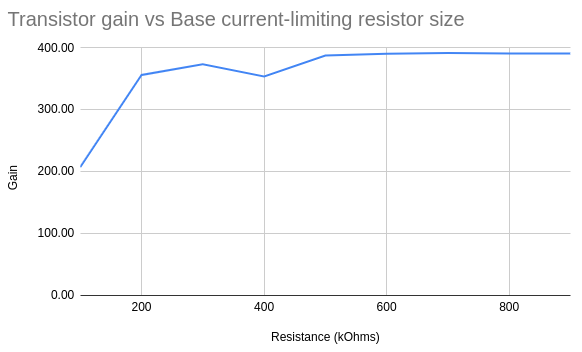
\includegraphics[width=0.6\textwidth]{gain.png}}
\end{center}
\vspace{-20pt}
\caption{Transistor gain vs Base limiting transistor }
\end{wrapfigure}
\\
It can also be noted form figure 2 that as the base current limiting resistor increases in size, the gain of the transistor increases,meaning that for the highest gain value, a large resistor must be used.\\\\\\

\section{Base current vs Collector current}

\begin{figure}[h]
 \begin{center}
  \fbox{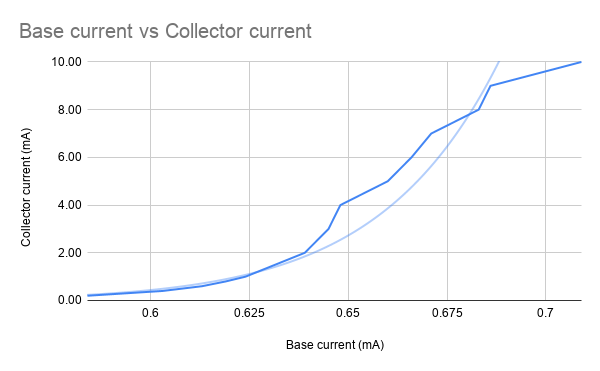
\includegraphics[width = 0.8\textwidth]{I_C.png}}
  \vspace{-8pt}
  \caption{Base current vs Collector current}
 \end{center}
\end{figure}

It can be observed in figure 3 that as the base current ($I_B$) increases, the collector current ($I_C$) will increase at an exponential rate. this means that with a relatively low base current, a large collector current can be allowed to flow. This is the basis of the amplification properties of transistors. 



\end{document}

\begin{figure}[h]
\begin{center}
\fbox{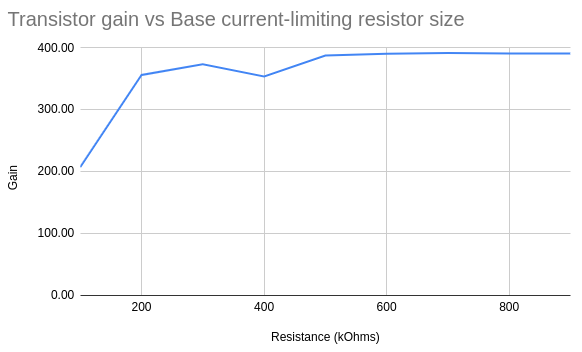
\includegraphics[width=0.5\textwidth]{gain.png}}
\end{center}
\caption{BJT Diode Model}
\end{figure}